\documentclass[article,A4,12pt]{llncs}
\usepackage[T1]{fontenc}
\usepackage{amsmath}
\usepackage{amssymb}
\usepackage{amsfonts}
\usepackage{mathrsfs, bm}

\usepackage{graphicx}
\usepackage{tabularx}
\usepackage{subfig}
\usepackage{epsf,times}
\usepackage{color}
\usepackage{wrapfig}
\usepackage{cases}
\usepackage{multicol}

\usepackage[T1]{fontenc}
%\newcommand{\tmname}[1]{\textsc{#1}}
%\newcommand{\tmop}[1]{\ensuremath{\operatorname{#1}}}
%\newcommand{\tmsamp}[1]{\textsf{#1}}
%\newcommand{\tmtextsc}[1]{{\scshape{#1}}}
%\newcommand{\tmtextsl}[1]{{\slshape{#1}}}
%\newcommand{\tmtexttt}[1]{{\ttfamily{#1}}}

\leftmargin=0.0cm
\oddsidemargin=0.5cm
\evensidemargin=0.5cm
\topmargin=0cm
\textwidth=16.0cm
%\textheight=21.5cm
\textheight=20.0cm
\pagestyle{plain}
\setlength{\columnsep}{20pt}

\def\m{\mathbf{m}}
\def\H{\mathbf{H}}
\def\E{\mathbf{E}}
\newcommand{\vepsi}{{\varepsilon}}
\def\hnorm#1#2{\vert\,#1\,\vert_{#2}}
\newcommand{\R}{{\mathbb R}}
\newcommand{\Sph}{{\mathbb S}}
\def\x{\mathbf{x}}
\def\hvec{\overline{\mathbf{h}}}
\def\evec{\overline{\mathbf{e}}}

\newcommand{ \etal}{\mbox{\emph{et al. }}}

\newcommand\vect[1]{\mbf{#1}}
\newcommand{\mbf}[1]{\mbox{\boldmath$#1$}} 
\newcommand{\RC}[1]{#1 $\times$ #1 $\times$ #1}
\def\um{$\mu$m}
\def\C{$^{\circ}\mathrm{C}$}

\newcommand{\Rmnum}[1]{\expandafter\@slowromancap\romannumeral #1@}

% DEFINITION OF CUSTOM FONT SIZE
\newcommand{\customfontA}{\fontsize{50}{55}\selectfont}
\newcommand{\customfontB}{\fontsize{14.4}{20}\selectfont}
\newcommand{\customfontC}{\fontsize{30}{35}\selectfont}

\DeclareMathAlphabet{\mathpzc}{OT1}{pzc}{m}{it}

\def\clovek#1{\noindent\bgroup\vbox{\noindent#1}\egroup\vskip1em}

% TO INPUT BACKGROUND IMAGE
\usepackage{eso-pic}
\newcommand\BackgroundPic{
\put(0,0){
\parbox[b][\paperheight]{\paperwidth}{
\vfill
\centering
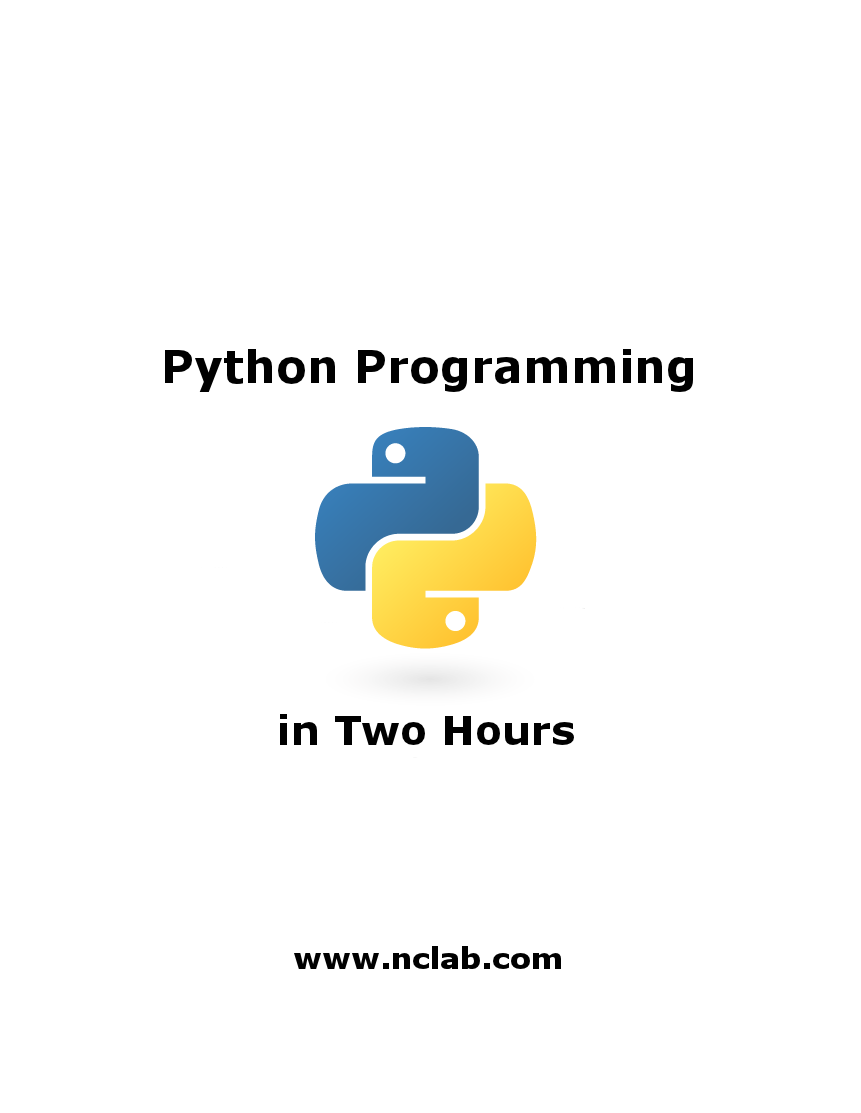
\includegraphics[width=\paperwidth,height=\paperheight]{img/python-frontpage.png}
%\includegraphics[width=\paperwidth,height=\paperheight]{img/background.jpg}
\vfill
}}}

\begin{document}

% INPUTTING BACKGROUND IMAGE
\AddToShipoutPicture{\BackgroundPic}
\vbox{}
\pagestyle{empty}
\newpage
\textwidth=15.5cm
\ClearShipoutPicture
\newpage

%%%%%%%%%%%%%%%%%%%%%%%%%%%%%%%%%%%%%%%%%%%%%%%%%%%%%%%%%%%%%%%%%%%%%%%%%

\section*{}
\small
\subsection*{About NCLab}
Networked Computing Laboratory (NCLab) is a popular Internet-based framework for 
programming, mathematics, computer modeling, 
and scientific computing. It serves students, instructors, researchers, and the general 
public. NCLab can be used free of charge for personal non-commercial purposes such as 
private hobby or self-education, as well as for individual non-funded academic research.
All other use is subject to {\bf purchasing a license} for a symbolic fee. The fees are as low as 
\$1 per user per month for educational use, and they are used to support the development 
and operational expenses. NCLab is a product of FEMhub Inc. The name "NCLab" is 
registered with the U.S. Patent and Trademark Office (USPTO) under Trademark No. 85420518.

\subsection*{Terms of Use and Pricing}
More details on purchasing a license and using NCLab are provided in the online documents 
{\bf Pricing} and {\bf Terms of Use} that are accessible from NCLab's home page 
{\tt http://nclab.com}.

\subsection*{Contact Information}
General inquiries: {\tt info@femhub.com}\\
Sales: {\tt sales@femhub.com}\\
NCLab support: {\tt support@nclab.com}\\
Agros \& Hermes support: {\tt support@femhub.com}\\
Web page: {\tt http://femhub.com}\\
{Physical address}\\
FEMhub Inc.\\
5490 Twin Creeks Dr.\\
Reno, NV 89523

\subsection*{About This Publication}
This publication can be copied and distributed without any restrictions
as long as reference to NCLab and FEMhub Inc. is preserved.

\subsection*{Acknowledgement}
This publication was created with the help of many freely 
available web resources related to Python, in
particular www.python.org.

\normalsize

\newpage
%{\ }
\setcounter{tocdepth}{2}
\tableofcontents
%\pagestyle{plain}

\newpage

\pagestyle{plain}
\setcounter{page}{1}

%%%%%%%%%%%%%%%%%%%%%%%%%%%%%%%%%%%%%%%%%%%%%%%%%%%%%%%%%%%%%%%%%%%%%%%%%

\section{Introduction}

Python is an easy to learn, powerful programming language. It has efficient high-level 
data structures and a simple but effective approach to object-oriented programming. 
Python's elegant syntax and dynamic typing, together with its interpreted nature, 
make it an ideal language for scripting and rapid application development in many 
areas on most platforms. 

Python is an {\em interpreted language} which means that commands are executed one by one 
in the order specified in the program. This is very different from {\em compiled languages}
such as C, C++ or Fortran where the entire program needs to be compiled first, and only
then it can be run. 

In order to make the most of this tutorial, we invite the 
reader to create an account in NCLab and log in. More instructions 
on how to do this are given at the beginning of the introductory 
tutorial "Meet Your New Graphing Calculator" that is available in 
PDF via a link on NCLab home page {\tt http://nclab.com}.
After login, you will see a desktop with several icons on it,
as shown in Fig. \ref{fig:desktop}. 


\begin{figure}[!ht]
\begin{center}
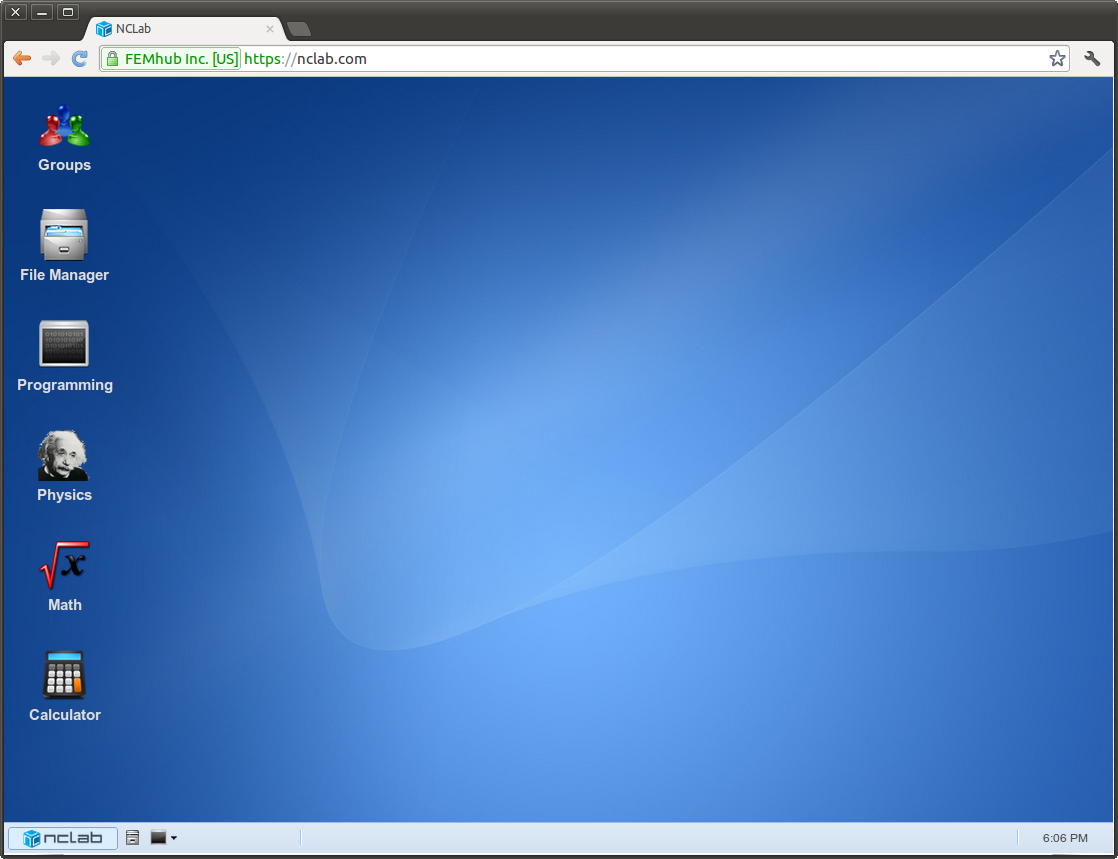
\includegraphics[width=\textwidth]{img/desktop.png}
\end{center}
\vspace{-2mm}
\caption{NCLab desktop after login.}
\label{fig:desktop}
\end{figure}
\newpage

\subsection*{Cloning Displayed Projects vs. Typing the Code by Yourself}

All examples that we are going to work with in the following are also available 
as Displayed Projects. This means that you can clone them by launching the File
Manager, going to the {\em Project} menu, and clicking on {\em Clone}. This will launch 
a window with many displayed projects from various areas of programming,
math and computing. Look for projects whose names start with "Tutorial - Python".
After you locate a project that you would like to clone, click on it,
and then click on the button {\em Clone} at the bottom of the window. This will
create exact copy of that project in your account, and you can open it 
by clicking on it in the File Manager. You can change the project in any way 
you like, the changes will not affect the original Displayed Project. 

Alternatively, you can type the examples by yourself, which is the 
recommended way. What you do with your own hands will come back much easier 
when you do it again. And moreover, the introductory examples have no more than 
a couple of lines anyway. So, in the File Manager's {\em Project} menu 
choose {\em New} $\rightarrow$ {\em Python}. This will launch an 
empty Python project, as shown in Fig. \ref{fig:python}.\\[-7mm]


\begin{figure}[!ht]
\begin{center}
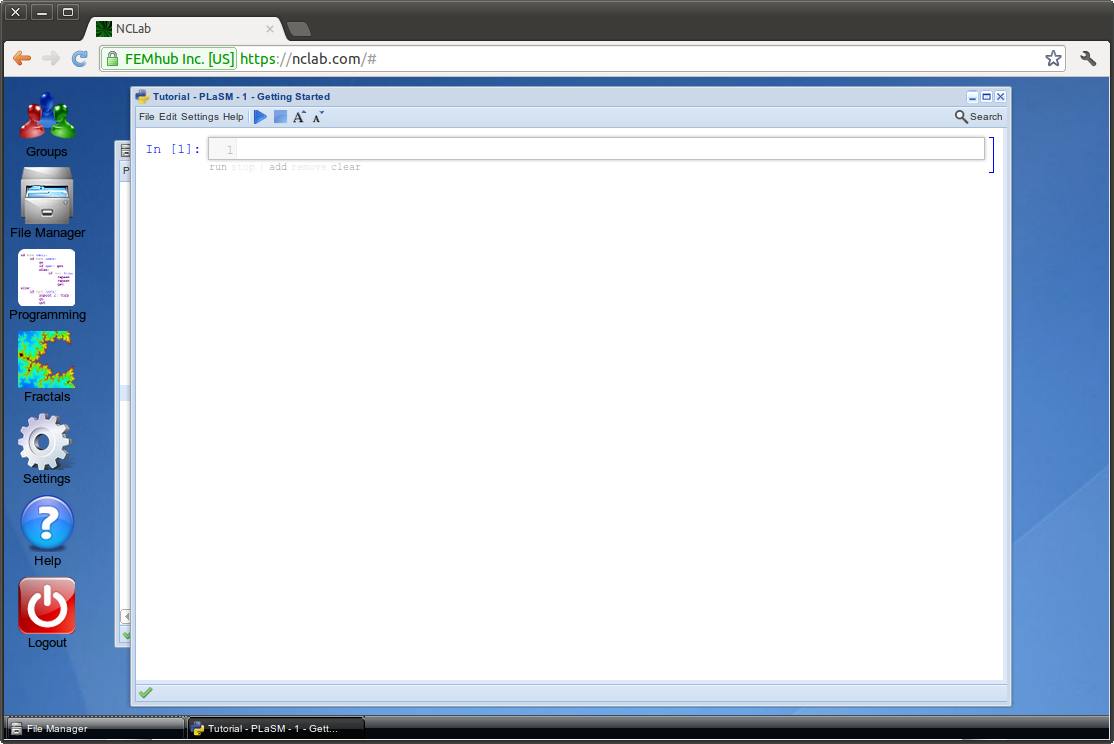
\includegraphics[width=\textwidth]{img/python.png}
\end{center}
\vspace{-2mm}
\caption{Launching a new Python project.}
\label{fig:python}
\end{figure}
\vspace{-1cm}
\noindent
\newpage




\section{Two-Hour Course}

Let us start with a two-hour course that consists of 10 short lessons. Thanks to the 
simplicity of Python, after this course you will be able to write a wide range of 
programs. Perhaps this course is all you will ever need. More advanced topics and 
object-oriented programming will follow in Sections
\ref{sec:adv} and \ref{sec:obj}, respectively.

\subsection{Lesson 1: Hello, World!}

Click into the input cell and type:

\begin{verbatim}
print "Hello, World!"
\end{verbatim}
Then click on the "run" link under the input cell and your program will be sent to the 
cloud. The response should come back instantly, and it should be displayed 
in a new yellow {\em output cell}:

\begin{verbatim}
Hello, World!
\end{verbatim}
You just learned the first Python command. This is the end of Lesson 1. Wasn't that simple?

\subsection{Lesson 2: Numbers}

The Python input cell can be used as a calculator. Try it and type 

\begin{verbatim}
3 + 6
\end{verbatim}
The click on the "run" link under the input cell. (We will not repeat the last sentence 
in the following, since this is the same whenever we want to send the contents of the input 
cell to the cloud.) The output is

\begin{verbatim}
9
\end{verbatim}
You can add real numbers too,
\begin{verbatim}
3.2 + 6.31
\end{verbatim}
Output:

\begin{verbatim}
9.51
\end{verbatim}
Two numbers can be subtracted as follows,

\begin{verbatim}
7.5 - 2.1
\end{verbatim}
Output:

\begin{verbatim}
5.4
\end{verbatim}
Multiplication is done using the '{\tt *}' symbol as in

\begin{verbatim}
3 * 12
\end{verbatim}
Output:

\begin{verbatim}
36
\end{verbatim}
Of course, real numbers can be multiplied as well:

\begin{verbatim}
3.7 * 12.17
\end{verbatim}
Output:

\begin{verbatim}
45.029
\end{verbatim}
With division, we need to be a bit careful. Look at this:

\begin{verbatim}
30 / 5
\end{verbatim}
Output:

\begin{verbatim}
6
\end{verbatim}
And then look at this:

\begin{verbatim}
33 / 5
\end{verbatim}
Output:

\begin{verbatim}
6
\end{verbatim}
In all major computer languages including C, C++, Fortran, Python and 
others, {\bf the result of division of two integers is an integer}. 
So, when dividing two integers, everything behind the decimal point is lost.
In fact this is true also for addition, subtraction and multiplication 
but there it cannot cause any harm. 

In order to stay on the safe side, 
before you perform division of two numbers, always convert at least one of them
to a real number. This is simple: While {\tt 5} is an integer, {\tt 5.}
and {\tt 5.0} are reals. It is also possible to 
say {\tt float(5)}. In fact this is the best way since it also works for 
variables. Such as, when we are dividing {\tt a / b}, to make sure that 
the result will be correct also for integers, we type {\tt float(a) / b}. 
When at least one number is a real, then the result of the division is a real.   
Variables will be discussed shortly.

Sometimes we need to use exponents, such as in $2^4$. Python has a double-star
symbol {\tt **} for this:

\begin{verbatim}
2**4
\end{verbatim}
Output:

\begin{verbatim}
16
\end{verbatim}
The last of the common arithmetic operations is {\em modulo}. Recall that this is the remainder 
after integer division. In Python modulo is done using the per cent symbol:

\begin{verbatim}
6 % 4
\end{verbatim}
Output:

\begin{verbatim}
2
\end{verbatim}
Of course, one can use brackets:

\begin{verbatim}
5 * (7 - 3)
\end{verbatim}
Output:

\begin{verbatim}
20
\end{verbatim}
Python respects the standard order of operations:

\begin{itemize} 
\item Brackets have the highest priority, 
\item then exponentiation, 
\item then multiplication and division (same priority),
\item the lowest priority have addition and subtraction.
\end{itemize}
To illustrate this, we can try the following:

\begin{verbatim}
3**4/27*5+3*5
\end{verbatim}
Output:

\begin{verbatim}
30
\end{verbatim}
Let us remark that your code will be much more readable when you use empty
characters on either side of arithmetic symbols. Hence instead of the 
previous compact expression you should write {\tt 3**4 / 27 * 5 + 3 * 5}.

Complex numbers are always represented as two floating point numbers, the 
real and imaginary part. Appending '{\tt j}' or  '{\tt J}' to a real number
makes it imaginary:

\begin{verbatim}
1j * 1J
\end{verbatim}
Output:

\begin{verbatim}
(-1+0j)
\end{verbatim}
This is one way to define complex numbers:
\begin{verbatim}
1 + 3j
\end{verbatim}
Output:

\begin{verbatim}
(1+3j)
\end{verbatim}
Another way is to use the command {\tt complex}:

\begin{verbatim}
complex(1, 3)
\end{verbatim}
Output:

\begin{verbatim}
(1+3j)
\end{verbatim}
All arithmetic operations that are used for real numbers can be 
used for complex numbers as well, for example:

\begin{verbatim}
(1 + 2j) / (1 + 1j)
\end{verbatim}
Output:

\begin{verbatim}
(1.5+0.5j)
\end{verbatim}
To extract the real and imaginary parts of a complex number {\tt z}, use {\tt z.real}
and {\tt z.imag}. Use {\tt abs()} to get the absolute value:

\begin{verbatim}
a = 3 + 4j
a.real
a.imag
abs(a)
\end{verbatim}
Output:

\begin{verbatim}
3
4
5
\end{verbatim}
Good job, now you know your numbers. This is the end of Lesson 2!


\subsection{Lesson 3: Variables}

In Python (and other languages as well) the symbol '{\tt =}' is used to assign 
a value to a variable. This operation does not produce any output. For
example:

\begin{verbatim}
width = 20
height = 5*5
\end{verbatim}
Output:

\begin{verbatim}

\end{verbatim}
(Yes, there is none!) If we want to see the values, we need to print the 
variables. To do this, it suffices to type the variable's name:

\begin{verbatim}
width
height
\end{verbatim}
Output:

\begin{verbatim}
20
25
\end{verbatim}
Or, we can use the print command:

\begin{verbatim}
print width
print height
\end{verbatim}
Output:

\begin{verbatim}
20
25
\end{verbatim}
The output can be made more informative (strongly encouraged!):

\begin{verbatim}
print "The width of the object is", width
print "And its height is", height
\end{verbatim}
Output:

\begin{verbatim}
The width of the object is 20
And its height is 25
\end{verbatim}
A value can be assigned to several variables at the same time:

\begin{verbatim}
x = y = z = 0.0
x
y
z
\end{verbatim}
Output:

\begin{verbatim}
0.0
0.0
0.0
\end{verbatim}
Variables must be defined (have a value assigned) before they can be 
used. For example, when trying to print a variable {\tt value} that 
was never used before, we get an error:

\begin{verbatim}
Traceback (most recent call last):
  File "<nclab>", line 1, in <module>
NameError: name 'value' is not defined
\end{verbatim}
The simplest way to increase the value of a variable by a given number is to use the '{\tt +=}' 
command:

\begin{verbatim}
v = 1
v += 3
print v
\end{verbatim}
Output:

\begin{verbatim}
4
\end{verbatim}
We can also subtract a number from a variable:

\begin{verbatim}
print v -= 1
\end{verbatim}
Output:

\begin{verbatim}
3
\end{verbatim}
We can multiply a variable with a number:

\begin{verbatim}
print v *= 4
\end{verbatim}
Output:

\begin{verbatim}
12
\end{verbatim}
And finally, we can divide a variable with a number:

\begin{verbatim}
print v /= 6
\end{verbatim}
Output:

\begin{verbatim}
2
\end{verbatim}
It is possible to use existing variables to assign a value to a new variable:

\begin{verbatim}
a = 1
b = 2.5
c = 0.5
d = (a + b) / c
d
\end{verbatim}
Output:

\begin{verbatim}
7.0
\end{verbatim}
And this lucky number means the end of Lesson 3!

\subsection{Lesson 4: Strings}

By a {\em string} we mean a text surrounded by double or single quotes, such as 
{\tt "this is a string"} or {\tt 'and this is a string as well'}.
Strings are useful to make outputs more informative, but 
they have many other uses as well. For example, they can represent data 
in databases such as in a phone book. So we need to understand them well,
as well as various operations that we can do with them.

Let us first understand how to use quotes in strings. The safest way is to use 
them with a backslash:

\begin{verbatim}
"I said \"yes\"."
\end{verbatim}
Output:

\begin{verbatim}
'I said "yes".'
\end{verbatim}
Another example:

\begin{verbatim}
"It doesn\'t matter."
\end{verbatim}
Output:

\begin{verbatim}
"It doesn't matter."
\end{verbatim}
When we want to use multi-line strings, the best way is to enclose them 
in triple quotes:

\begin{verbatim}
edgar = """
Once upon a midnight dreary, while I pondered weak and weary,
Over many a quaint and curious volume of forgotten lore,
While I nodded, nearly napping, suddenly there came a tapping,
As of some one gently rapping, rapping at my chamber door.
`'Tis some visitor,' I muttered, `tapping at my chamber door -
Only this, and nothing more.'
"""
print edgar
\end{verbatim}
Output:

\begin{verbatim}
Once upon a midnight dreary, while I pondered weak and weary,
Over many a quaint and curious volume of forgotten lore,
While I nodded, nearly napping, suddenly there came a tapping,
As of some one gently rapping, rapping at my chamber door.
`'Tis some visitor,' I muttered, `tapping at my chamber door -
Only this, and nothing more.'
\end{verbatim}
Strings can be concatenated (glued together) with the '{\tt +}' operator, and repeated with '{\tt *}':

\begin{verbatim}
word = 'Help' + 'me!'
print "I yelled" + 3 * word
\end{verbatim}
Output:

\begin{verbatim}
I yelledHelpme!Helpme!Helpme!
\end{verbatim}
You can see that empty spaces matter. Let's try again:

\begin{verbatim}
word = '\"Help' + ' me!\" '
print "I yelled " + 3 * word
\end{verbatim}
Output:

\begin{verbatim}
I yelled "Help me!" "Help me!" "Help me!"
\end{verbatim}
Individual letters forming a string can be accessed via indices. The indices 
start from zero, as in C and C++. It is also handy to use the index {\tt -1} 
for the last index, {\tt -2} for the one-before-last etc.


\begin{verbatim}
word = "breakfast"
print "First character:", word[0]
print "Second character:", word[1]
print "Last character:", word[-1]
print "One-before-last character:", word[-2]
\end{verbatim}
Output:

\begin{verbatim}
First character: b
Second character: r
Last character: t
One-before-last character: s
\end{verbatim}
We can also access substrings, this is called {\em slicing}:

\begin{verbatim}
w1 = "bicycle"
w2 = w1[0:3]
print w2
\end{verbatim}
Output:

\begin{verbatim}
bic
\end{verbatim}
An omitted first index in a slice defaults to zero:

\begin{verbatim}
w3 = w1[0:2]
print w3
\end{verbatim}
Output:

\begin{verbatim}
bi
\end{verbatim}
An omitted second index defaults to the length of the string:

\begin{verbatim}
w4 = w1[2:]
print w4
\end{verbatim}
Output:

\begin{verbatim}
cycle
\end{verbatim}
And by the way, the length of a string can be obtained via the {\tt len()} function:

\begin{verbatim}
print len(w1)
\end{verbatim}
Output:

\begin{verbatim}
7
\end{verbatim}
Perhaps this lesson could be longer but it isn't. This concludes Lesson 4!


\subsection{Lesson 5: Conditions and the {\tt while} loop}




\subsection{Lesson 6: Defining new functions}






\subsection{Lesson 7: Tuples, lists, dictionaries}







\subsection{Lesson 8: The {\tt for} loop}



\subsection{Lesson 9: Classes - the basics}


\subsection{Lesson 10: Using libraries}



\section{Advanced Topics} \label{sec:adv}


\subsection{The {\tt break} and {\tt continue} statements}



\subsection{The {\tt else} clause for loops}



\subsection{The {\tt pass} statement}






\subsection{Default argument values}


\subsection{Keyword arguments}


\subsection{Arbitrary argument lists}


\subsection{Unpacking argument lists}


\subsection{Lambda forms}


\subsection{Documentation strings}




\subsection{Using lists as stacks}


\subsection{Using lists as queues}


\subsection{Functional programming tools}


\subsection{List comprehensions}


\subsection{The {\tt del} statement}


\subsection{Tuples and sequences}


\subsection{Sets}


\subsection{Dictionaries}


\subsection{Looping techniques}


\subsection{Input and output}


\subsection{Errors and Exceptions}


\subsection{Syntax errors}


\subsection{Exceptions}


\subsection{Handling exceptions}


\subsection{Raising exceptions}


\subsection{User-defined exceptions}


\subsection{Defining clean-up actions}


\section{Object-Oriented Programming} \label{sec:obj}


\subsection{Inheritance}


\subsection{Private variables}


\subsection{Iterators}


\subsection{Generators}










\end{document}
